%%%%%%%%%%%%%%%%%%%%%%%%%%%%%%%%%%%%%%%%%%%%%%%%%%%%%%%%%%%%%%%%%%%%%%
%%                     Omitted Process
%%%%%%%%%%%%%%%%%%%%%%%%%%%%%%%%%%%%%%%%%%%%%%%%%%%%%%%%%%%%%%%%%%%%%%
%\color{blue}
\subsection{Glyph: \glyph{Omitted process}}\label{sec:omitted}

Omitted processes are processes that are known to exist, but are omitted from the map for the sake of clarity or parsimony. A single \glyph{omitted process} can represent any number of actual processes. The \glyph{omitted process} is different from a \glyph{submap}. While a \glyph{submap} references to an explicit content, that is hidden in the main map, the \glyph{omitted process} does not ``hide'' anything within the context of the map, and cannot be ``unfolded''.

\begin{glyphDescription}
 \glyphSboTerm SBO:0000397 - omitted process.
 \glyphOrigin One or several \glyph{consumption} arcs (\sect{consumption}) or one or several \glyph{production} arcs (\sect{production}).
 \glyphTarget One or several \glyph{production} arcs (\sect{production}).

 \glyphNode An \glyph{omitted process} is represented by a \glyph{process} in which the square box contains a two parallel slanted lines oriented northwest-to-southeast and separated by an empty space.
 \end{glyphDescription}

\begin{figure}[H]
  \centering
  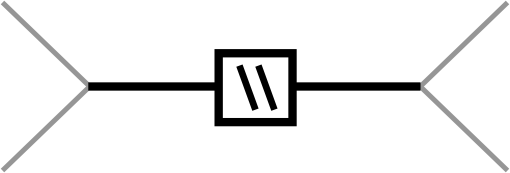
\includegraphics[scale = 0.5]{images/omitted}
  \caption{The \PD glyph for \glyph{omitted process}.}
  \label{fig:omitted}
\end{figure}



